%%%%%%%%%%%%%%%%%%%%%%%%%%%%%%%%%%%%%%%%%
% Lachaise Assignment
% LaTeX Template
% Version 1.0 (26/6/2018)
%
% This template originates from:
% http://www.LaTeXTemplates.com
%
% Authors:
% Marion Lachaise & François Févotte
% Vel (vel@LaTeXTemplates.com)
%
% License:
% CC BY-NC-SA 3.0 (http://creativecommons.org/licenses/by-nc-sa/3.0/)
% 
%%%%%%%%%%%%%%%%%%%%%%%%%%%%%%%%%%%%%%%%%

%----------------------------------------------------------------------------------------
%	PACKAGES AND OTHER DOCUMENT CONFIGURATIONS
%----------------------------------------------------------------------------------------

\documentclass{article}

%%%%%%%%%%%%%%%%%%%%%%%%%%%%%%%%%%%%%%%%%
% Lachaise Assignment
% Structure Specification File
% Version 1.0 (26/6/2018)
%
% This template originates from:
% http://www.LaTeXTemplates.com
%
% Authors:
% Marion Lachaise & François Févotte
% Vel (vel@LaTeXTemplates.com)
%
% License:
% CC BY-NC-SA 3.0 (http://creativecommons.org/licenses/by-nc-sa/3.0/)
% 
%%%%%%%%%%%%%%%%%%%%%%%%%%%%%%%%%%%%%%%%%

%----------------------------------------------------------------------------------------
%	PACKAGES AND OTHER DOCUMENT CONFIGURATIONS
%----------------------------------------------------------------------------------------

\usepackage{amsmath,amsfonts,stmaryrd,amssymb} % Math packages

\usepackage{enumerate} % Custom item numbers for enumerations

\usepackage[ruled]{algorithm2e} % Algorithms

\usepackage[framemethod=tikz]{mdframed} % Allows defining custom boxed/framed environments

\usepackage{listings} % File listings, with syntax highlighting
\lstset{
	basicstyle=\ttfamily, % Typeset listings in monospace font
}

%----------------------------------------------------------------------------------------
%	DOCUMENT MARGINS
%----------------------------------------------------------------------------------------

\usepackage{geometry} % Required for adjusting page dimensions and margins

\geometry{
	paper=a4paper, % Paper size, change to letterpaper for US letter size
	top=2.5cm, % Top margin
	bottom=3cm, % Bottom margin
	left=2.5cm, % Left margin
	right=2.5cm, % Right margin
	headheight=14pt, % Header height
	footskip=1.5cm, % Space from the bottom margin to the baseline of the footer
	headsep=1.2cm, % Space from the top margin to the baseline of the header
	%showframe, % Uncomment to show how the type block is set on the page
}

%----------------------------------------------------------------------------------------
%	FONTS
%----------------------------------------------------------------------------------------

\usepackage[utf8]{inputenc} % Required for inputting international characters
\usepackage[T1]{fontenc} % Output font encoding for international characters

\usepackage{XCharter} % Use the XCharter fonts

%----------------------------------------------------------------------------------------
%	COMMAND LINE ENVIRONMENT
%----------------------------------------------------------------------------------------

% Usage:
% \begin{commandline}
%	\begin{verbatim}
%		$ ls
%		
%		Applications	Desktop	...
%	\end{verbatim}
% \end{commandline}

\mdfdefinestyle{commandline}{
	leftmargin=10pt,
	rightmargin=10pt,
	innerleftmargin=15pt,
	middlelinecolor=black!50!white,
	middlelinewidth=2pt,
	frametitlerule=false,
	backgroundcolor=black!5!white,
	frametitle={Command Line},
	frametitlefont={\normalfont\sffamily\color{white}\hspace{-1em}},
	frametitlebackgroundcolor=black!50!white,
	nobreak,
}

% Define a custom environment for command-line snapshots
\newenvironment{commandline}{
	\medskip
	\begin{mdframed}[style=commandline]
}{
	\end{mdframed}
	\medskip
}

%----------------------------------------------------------------------------------------
%	FILE CONTENTS ENVIRONMENT
%----------------------------------------------------------------------------------------

% Usage:
% \begin{file}[optional filename, defaults to "File"]
%	File contents, for example, with a listings environment
% \end{file}

\mdfdefinestyle{file}{
	innertopmargin=1.6\baselineskip,
	innerbottommargin=0.8\baselineskip,
	topline=false, bottomline=false,
	leftline=false, rightline=false,
	leftmargin=2cm,
	rightmargin=2cm,
	singleextra={%
		\draw[fill=black!10!white](P)++(0,-1.2em)rectangle(P-|O);
		\node[anchor=north west]
		at(P-|O){\ttfamily\mdfilename};
		%
		\def\l{3em}
		\draw(O-|P)++(-\l,0)--++(\l,\l)--(P)--(P-|O)--(O)--cycle;
		\draw(O-|P)++(-\l,0)--++(0,\l)--++(\l,0);
	},
	nobreak,
}

% Define a custom environment for file contents
\newenvironment{file}[1][File]{ % Set the default filename to "File"
	\medskip
	\newcommand{\mdfilename}{#1}
	\begin{mdframed}[style=file]
}{
	\end{mdframed}
	\medskip
}

%----------------------------------------------------------------------------------------
%	NUMBERED QUESTIONS ENVIRONMENT
%----------------------------------------------------------------------------------------

% Usage:
% \begin{question}[optional title]
%	Question contents
% \end{question}

\mdfdefinestyle{question}{
	innertopmargin=1.2\baselineskip,
	innerbottommargin=0.8\baselineskip,
	roundcorner=5pt,
	nobreak,
	singleextra={%
		\draw(P-|O)node[xshift=1em,anchor=west,fill=white,draw,rounded corners=5pt]{%
		Question \theQuestion\questionTitle};
	},
}

\newcounter{Question} % Stores the current question number that gets iterated with each new question

% Define a custom environment for numbered questions
\newenvironment{question}[1][\unskip]{
	\bigskip
	\stepcounter{Question}
	\newcommand{\questionTitle}{~#1}
	\begin{mdframed}[style=question]
}{
	\end{mdframed}
	\medskip
}

%----------------------------------------------------------------------------------------
%	WARNING TEXT ENVIRONMENT
%----------------------------------------------------------------------------------------

% Usage:
% \begin{warn}[optional title, defaults to "Warning:"]
%	Contents
% \end{warn}

\mdfdefinestyle{warning}{
	topline=false, bottomline=false,
	leftline=false, rightline=false,
	nobreak,
	singleextra={%
		\draw(P-|O)++(-0.5em,0)node(tmp1){};
		\draw(P-|O)++(0.5em,0)node(tmp2){};
		\fill[black,rotate around={45:(P-|O)}](tmp1)rectangle(tmp2);
		\node at(P-|O){\color{white}\scriptsize\bf !};
		\draw[very thick](P-|O)++(0,-1em)--(O);%--(O-|P);
	}
}

% Define a custom environment for warning text
\newenvironment{warn}[1][Warning:]{ % Set the default warning to "Warning:"
	\medskip
	\begin{mdframed}[style=warning]
		\noindent{\textbf{#1}}
}{
	\end{mdframed}
}

%----------------------------------------------------------------------------------------
%	INFORMATION ENVIRONMENT
%----------------------------------------------------------------------------------------

% Usage:
% \begin{info}[optional title, defaults to "Info:"]
% 	contents
% 	\end{info}

\mdfdefinestyle{info}{%
	topline=false, bottomline=false,
	leftline=false, rightline=false,
	nobreak,
	singleextra={%
		\fill[black](P-|O)circle[radius=0.4em];
		\node at(P-|O){\color{white}\scriptsize\bf i};
		\draw[very thick](P-|O)++(0,-0.8em)--(O);%--(O-|P);
	}
}

% Define a custom environment for information
\newenvironment{info}[1][Info:]{ % Set the default title to "Info:"
	\medskip
	\begin{mdframed}[style=info]
		\noindent{\textbf{#1}}
}{
	\end{mdframed}
}
 % Include the file specifying the document structure and custom commands

%----------------------------------------------------------------------------------------
%	ASSIGNMENT INFORMATION
%----------------------------------------------------------------------------------------

\title{Programming project - Graph Partitioning} % Title of the assignment

\author{
  Anssi Moisio\\
  \texttt{anssi.moisio@aalto.fi}
  \and
  Nikolas Erkinheimo\\
  \texttt{nikolas.erkinheimo@aalto.fi}
}

\date{Algorithmic Methods of Data Mining --- \today} % University, school and/or department name(s) and a date

%----------------------------------------------------------------------------------------

\begin{document}

\maketitle % Print the title

%----------------------------------------------------------------------------------------
%	INTRODUCTION
%----------------------------------------------------------------------------------------

\section*{Introduction} % Unnumbered section

The topic of this programming exercise is graph partitioning.
The datasets being used are provided by SNAP (Stanford Network Analysis project).
We will use the following five undirected networks:

\begin{itemize}
	\item ca-GrQc 
	\item Oregon-1
	\item soc-Epinions1
	\item web-NotreDame
	\item roadNet-CA
\end{itemize}

The networks have substantial size differences: the amount of vertices range from
about 4000 (ca-GrQc) to about 2000000 (roadNet-CA). We will be using mostly
the two smallest graphs when validating our algorithms to save time.
The graphs have defined values of k (numbers of clusters), that will be used in
the competition, from 2 to 50. We will use these same k values throughout the project.

Graph partitioning is a classical NP-hard problem which means polynomial time algorithms for this problem may not even exist and at the very least have not been found yet. We will use spectral algorithms. First, we will generate the Laplacian matrix of all of the graphs after which we calculate the corresponding eigenvectors. We will then apply a clustering algorithm to these eigenvectors to partition the nodes into sets.

We used the following loss function:

\begin{equation}
	\phi(V_1,...,V_k) = \frac{\lvert{E(V_i,...,V_k)}\rvert}{min_{1\leq{i}\leq{k}}\lvert{V_i}\rvert}
\end{equation}

Where the nominator corresponds to the amount of cut edges and the denominator is the size of the smallest cluster. 
%----------------------------------------------------------------------------------------
%	PROBLEM 1
%----------------------------------------------------------------------------------------

\section{Implementation} % Numbered section

We are using Python 3 as our implementation language along with the following packages: scikit-learn, networkx, numpy, scipy and pandas. We intend to use spectral algorithms for this problem.
%------------------------------------------------

\subsection{Data loading and preprocessing}

The data is in an edgelist format which will need to be loaded from the filesystem. We used pandas to load the files as DataFrames which we converted into adjacency matrices using networkx. We used scipy to morph the adjacency matrix into a normed Laplacian matrix.
	
%------------------------------------------------

\subsection{Clustering the eigenvectors}

Every row represents a node in the graph. Now that the graph has been converted into a matrix we can apply numerical algorithms to it. We used k-means to cluster the eigenvectors into sets and calculated the loss function.
%----------------------------------------------------------------------------------------
%	PROBLEM 2
%----------------------------------------------------------------------------------------

\section{Results}
Kuvaajat: 
\begin{itemize}
	\item ${\phi(max\ iters)}$
	\item ${\phi_{min}(number\ of\ sampled\ kmeans\ results)}$
	\item Effect of normalization on results
\end{itemize}

\begin{figure}[htb]

\begin{center} 
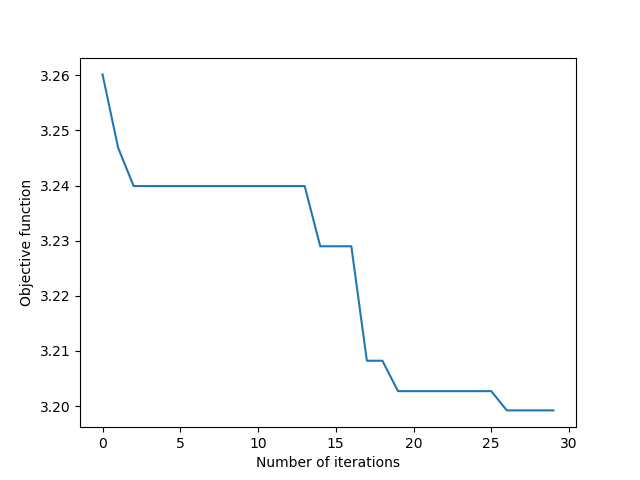
\includegraphics[height=10cm]{plot2.png}
\end{center}
\caption{The objective function as a function of the number of iterations of the algorithm.
The eigenvectors are normalized here. This figure is for the smallest graph ca-GrQc, with k=2.}
\label{plot1}
\end{figure}

From Figure \ref{plot1} we can see that iterating the algorithm with
new initializations can make the results better. For the smallest
network the differences are not large (from 3.26 to 3.20) but with the
larger networks there is noticeable differences (see Figure \ref{normalized2}).

\begin{figure}[htb]
\begin{center} 
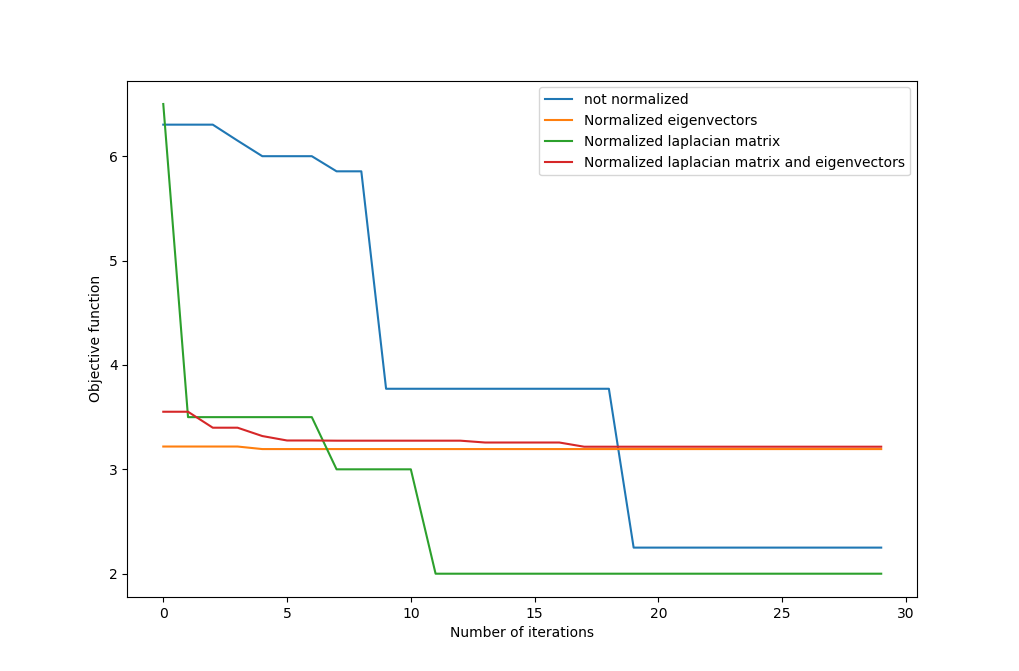
\includegraphics[height=12cm]{normalization_plot.png}
\end{center}
\caption{Results for normalized eigenvectors or Laplacian matrix or both
This figure is for the smallest graph ca-GrQc, with k=2.}
\label{normalized}
\end{figure}



From Figure \ref{normalized} we can see that normalizing the eigenvectors
makes the results stable. Normalizing the Laplacian matrix gives the best results and
normalizing the eigenvectors can actually make the results somewhat worse than
not normalizing anything.

\begin{figure}[htb]
\begin{center} 
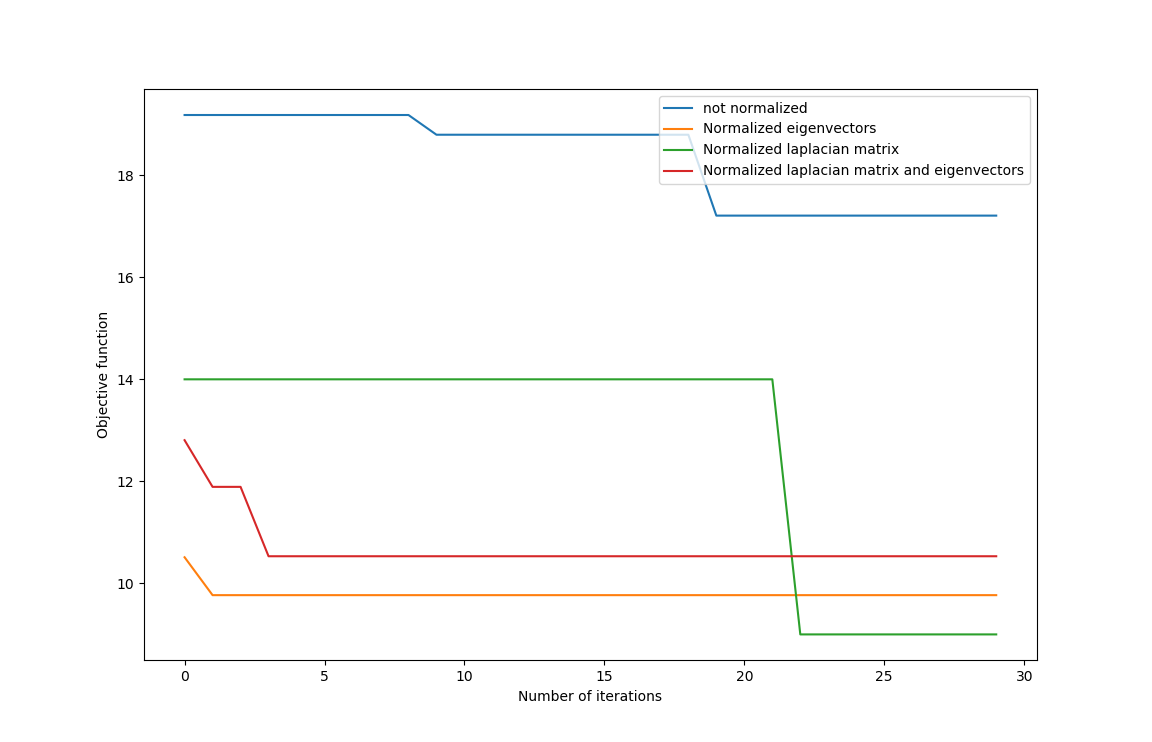
\includegraphics[height=12cm]{normalization_plot-oregonk5.png}
\end{center}
\caption{Results for normalized eigenvectors or Laplacian matrix or both.
This figure is for the second smallest graph Oregon-1, with k=5.}
\label{normalized2}
\end{figure}

\clearpage
\section{Conclusions}

Conclusions
%----------------------------------------------------------------------------------------

\end{document}
